\section{Method}
In this section we are going to first describe the approach followed towards model selection and model evaluation. Then, we will analyse the explored classification methods and the results they yielded.
 
\subsection{Approach}
In order to perform our analysis, we will adopt two approaches towards model selection:
\begin{itemize}
	\item \textbf{single split}: the training set is divided into two chunks, where the 80\% of the samples are used for fitting the classifer and the remaining 20\% for testing it. 
	\item \textbf{k-fold cross validation}: the training set is split into $k$ folds, one of whom is used for validation and the other $k - 1$ for fitting the model. The process is repeated $k$ times. This approach usually makes the process of model selection more reliable as, one by one, all the chunks will be used as unseen data. 
	For this specific application, we set $k = 5$, i.e. we used 5 folds. 
	
\end{itemize}
In both cases, we make sure no transformation is applied on the whole training data before splitting it, \textbf{not} to \textbf{bias} the validation and introduce \textbf{data leakages}.  

As regards model evalution, we want to be Bayesian and adopt the minimum of the normalized Bayesian risk as metric, which measures the cost we would pay if we made optimal decisions using the recognizer scores. The application of interest is a uniform prior one
\begin{align*}
	(\tilde{\pi}, C_{fp}, C_{fn}) = (0.5, 1, 1)
\end{align*}

being $\tilde{\pi}$ the (unbiased, in the specified case) prior, $C_{fp}, C_{fn}$ the costs of the false positive and false negative case, respectively. This is the case we will analyze extensively.  However, we also consider biased cases towards one of the qualities
\begin{align*}
	(\tilde{\pi}, C_{fp}, C_{fn}) = (0.1, 1, 1) \\
	(\tilde{\pi}, C_{fp}, C_{fn}) = (0.9, 1, 1)
\end{align*}


%%%%%%%%%%%%%%%%%%%%%%%%%%%%%%%%%%%%%%%%%%%%
%% Gaussian Classifiers
%%%%%%%%%%%%%%%%%%%%%%%%%%%%%%%%%%%%%%%%%%%%
\subsection{Gaussian Classifiers}

Gaussian classifiers are the first class of methods we take into considerations. In particular we analyse the performances yielded by a Multivariate Gaussian and a Naive Bayes, both with full and tied covariance, for a total of 4 classifiers.
 
Table \ref{tab:gaus_res} shows the results obtained for these models both for the single split and for the k-fold cross validation on raw and gaussianized data and applying PCA.


\begin{table}[H]
	\resizebox{.5\textwidth}{!}{
		\begin{tabular}{ p{2.5cm} p{1.5cm} p{1.5cm} p{1.5cm}}	
			\hline
			\hline
			\multicolumn{3}{c}{\hfill \textbf{single-split} \hfill} \\
			
			& $\tilde{\pi}=0.1$ & $\tilde{\pi}=0.5$
			& $\tilde{\pi}=0.9$ \\
			\hline
			\multicolumn{3}{c}{\hfill Raw features \hfill} \\
			\hline
			Full-Cov 	  & \boxit{red}{.35in}0.702 &  0.264 & 0.802\\
			Diag-Cov 	  & 0.822 & 0.409 & 0.941\\
			Tied Full-Cov & 0.754 & 0.327 & 0.706 \\
			Tied Diag-Cov & 0.820 & 0.391 & 0.908\\	
			\hline
			\multicolumn{3}{c}{\hfill Gaussianized features \hfill} \\
			\hline
			Full-Cov      & 0.761 &  0.255 & 0.729\\
			Diag-Cov      & 0.840 & 0.460 & 0.866\\
			Tied Full-Cov & 0.726 & 0.344 & 0.797 \\
			Tied Diag-Cov & 0.834 & 0.441 & 0.928\\	
			\hline
			\multicolumn{3}{c}{\hfill Gaussianized features, PCA(m=10) \hfill} \\
			\hline
			Full-Cov      & 0.726 &  \boxit{red}{.35in}0.242 & \boxit{red}{.35in}0.655\\
			Diag-Cov      & \boxit{cyan}{.35in}0.707 & 0.372 & 0.789\\
			Tied Full-Cov & 0.709 & 0.359 & 0.698 \\
			Tied Diag-Cov & 0.709 & 0.362 & 0.710\\
			\hline
			\multicolumn{3}{c}{\hfill Gaussianized features, PCA(m=9) \hfill} \\
			\hline
			Full-Cov      & 0.740 &  0.253 & 0.698\\
			Diag-Cov      & 0.720 & 0.384 & 0.790\\
			Tied Full-Cov & 0.719 & 0.361 & 0.731 \\
			Tied Diag-Cov & 0.726 & 0.361 & 0.746\\	
			\hline	
		\end{tabular}
	}

	\resizebox{.5\textwidth}{!}{
	\begin{tabular}{ p{2.5cm} p{1.5cm} p{1.5cm} p{1.5cm}}	
		\hline
		\multicolumn{3}{c}{\hfill \textbf{5-fold} \hfill} \\
		
		& $\tilde{\pi}=0.1$ & $\tilde{\pi}=0.5$
		& $\tilde{\pi}=0.9$ \\
		\hline
		\multicolumn{3}{c}{\hfill Raw features \hfill} \\
		\hline
		Full-Cov 	  & \boxit{red}{.35in}0.781 & 0.312 & 0.842\\
		Diag-Cov 	  & 0.847 & 0.420 & 0.922\\
		Tied Full-Cov & 0.810 & 0.334 & 0.746 \\
		Tied Diag-Cov & 0.866 & 0.402 & 0.932\\	
		\hline
		\multicolumn{3}{c}{\hfill Gaussianized features \hfill} \\
		\hline
		Full-Cov 	  & 0.799 & 0.301 & 0.773\\
		Diag-Cov      & 0.848 & 0.440 & 0.872\\
		Tied Full-Cov & 0.791 & 0.348 & 0.856 \\
		Tied Diag-Cov & 0.869 & 0.441 & 0.940\\	
		\hline
		\multicolumn{3}{c}{\hfill Gaussianized features, PCA(m=10) \hfill} \\
		\hline
		Full-Cov 	  & \boxit{cyan}{.35in}0.789 & \boxit{red}{.35in}0.290 & \boxit{red}{.35in}0.715\\
		Diag-Cov 	  & 0.819 & 0.389 & 0.874\\
		Tied Full-Cov & 0.794 & 0.352 & 0.802 \\
		Tied Diag-Cov & 0.793 & 0.351 & 0.822\\
		\hline
		\multicolumn{3}{c}{\hfill Gaussianized features, PCA(m=9) \hfill} \\
		\hline
		Full-Cov 	  & 0.812 & 0.304 & \boxit{cyan}{.35in}0.716\\
		Diag-Cov 	  & 0.819 & 0.392 & 0.825\\
		Tied Full-Cov & 0.810 & 0.351 & 0.791 \\
		Tied Diag-Cov & 0.809 & 0.353 & 0.813\\	
		\hline	
	\end{tabular}
}
\caption{min DCF for Gaussian models for different values of $\tilde{\pi}$}
\label{tab:gaus_res}
\end{table}


We notice that the full-covariance Multivariate Gaussian classifier yields the better performances, both with and without PCA. In particular, the dimensionality reduction is beneficial when applyied with 10 components and doesn't degrade the performances with 9.

This suggests the dataset is large enough to estimate a covariance matrix for each class and loosening our assumptions (introducing diagonalization or tying) is not needed. This is furtherly suggested by the fact that the diagonal covariance models yield the worst results, as the uncorrelation hypotesis does not hold.

Eventually, it should be noted that, as expected, gaussianization improves the performances with respect to raw data. The results obtained for the single split and 5-fold are consistent to one another, conveying that, in this specific scenario, the size of our training set is appropriate even for a single fold evaluation (i.e. a single split).


%%%%%%%%%%%%%%%%%%%%%%%%%%%%%%%%%%%%%%%%%%%%
%% 		Logistic Regression
%%%%%%%%%%%%%%%%%%%%%%%%%%%%%%%%%%%%%%%%%%%%
\subsection{Logistic Regression}

In this section, we assess the performances of a Logistic Regression classifier, both with linear and quadratic kernel.

Being classes unbalanced, their costs are rebalanced using a loss function accounting for the number of samples for each class, used as weights for the two terms deriving from the split of the summation of the original loss

\begin{align*}
	J(w, b) &= \cfrac{\lambda}{2} \|w\|^2 + \cfrac{\pi_T}{n_T} \sum_{i|c_i=1} log \ \sigma(y_i)^{-1} 
	\\ &+ \cfrac{1 - \pi_T}{n_F} \sum^n_{i| c_i=0} log \ \sigma(y_i)^{-1} 
\end{align*}
being $\sigma(.)$ the sigmoid function, $y_i$ the output of the model $y_i = - z_i (w^T x_i + b)$, $z_i$ a variable equal to $\pm 1$ depending on the class, $w, b$ the parameters of the model. 

The most significant results obtained for both the models for different values of $\lambda$ are shown in Table \ref{tab:lr_res}, while a complete visualization  of both the models for the balanced prior is shown in Figure \ref{fig:lr_plot}. 
\noindent
\begin{table}[H]
	\resizebox{.5\textwidth}{!}{
	\begin{tabular}{ P{3.15cm} P{1.5cm} P{1.5cm} P{1.5cm}}
		\hline
		\hline
		\multicolumn{3}{c}{\hfill \textbf{single-split} } \\
		
			& $\tilde{\pi}=0.1$ & $\tilde{\pi}=0.5$
			& $\tilde{\pi}=0.9$ \\
		\hline
		\multicolumn{3}{c}{\hfill Raw features \hfill} \\
		\hline
		Log-Reg ($\lambda=10^{-4}$) & 0.743 & 0.364 & 0.677  \\
		Quad-LR ($\lambda=0$)       & 1.000 & 1.000 & 0.900 \\
		\hline
		\multicolumn{3}{c}{Z-normalized features} \\
		\hline
		Log-Reg($\lambda=10^{-2})$ & 0.753 & 0.353                   & 0.754 \\
		Quad-LR($\lambda=0$)      & 1.000 & \boxit{red}{.35in}0.237 & 0.488 \\	
		\hline
		\multicolumn{3}{c}{Gaussianized features} \\
		\hline
		Log-Reg($\lambda=0$)       & 0.758 & 0.335 & 0.724 \\
		Quad-LR($\lambda=10^{-2}$) & \boxit{red}{.35in}0.560 & 0.256 & \boxit{red}{.35in}0.395 \\	
		\hline
		\multicolumn{3}{c}{Z-normalized features, PCA(m=10)} \\
		\hline
		Log-Reg($\lambda=10^{-2}$) & 0.760 & 0.353 & 0.752  \\
		Quad-LR($\lambda=0$) 	   & 0.601 & 0.243 & 0.400  \\	
		\hline
	\end{tabular}
	}
	% k fold
	\resizebox{.5\textwidth}{!}{
	\begin{tabular}{ P{3.15cm} P{1.5cm} P{1.5cm} P{1.5cm}}
		\hline
		\multicolumn{3}{c}{\hfill \textbf{5-fold} } \\

		& $\tilde{\pi}=0.1$ & $\tilde{\pi}=0.5$
		& $\tilde{\pi}=0.9$ \\
		\hline
		\multicolumn{3}{c}{\hfill Raw features \hfill} \\
		\hline
		Log-Reg ($\lambda=10^{-4}$) & 0.826 & 0.355  & 0.670  \\
		Quad-LR ($\lambda=0$)       & 1.000 & 1.000  & 1.000 \\
		\hline
		\multicolumn{3}{c}{Z-normalized features} \\
		\hline
		Log-Reg($\lambda=10^{-2})$ & 0.834 & 0.343  &  0.670 \\
		Quad-LR($\lambda=0$)       & 0.764 & \boxit{red}{.35in}0.273  &  0.687\\	
		\hline
		\multicolumn{3}{c}{Gaussianized features} \\
		\hline
		Log-Reg($\lambda=0$)       & 0.825 &  0.354 &  0.727\\
		Quad-LR($\lambda=10^{-2}$) & \boxit{red}{.35in}0.679 &  0.289 &  \boxit{red}{.35in}0.590\\	
		\hline
		\multicolumn{3}{c}{Z-normalized features, PCA(m=10)} \\
		\hline
		Log-Reg($\lambda=10^{-2}$) & 0.834 &  0.348 &   0.670 \\
		Quad-LR($\lambda=0$) 	   & 0.759 &  0.280 &   0.678\\	
		\hline
	\end{tabular}
}
	\caption{min DCF for Logistic Regression models}
	\label{tab:lr_res}
\end{table}
%%
\begin{figure}[H]
    %\centering
	\subfloat[linear, 5-fold]{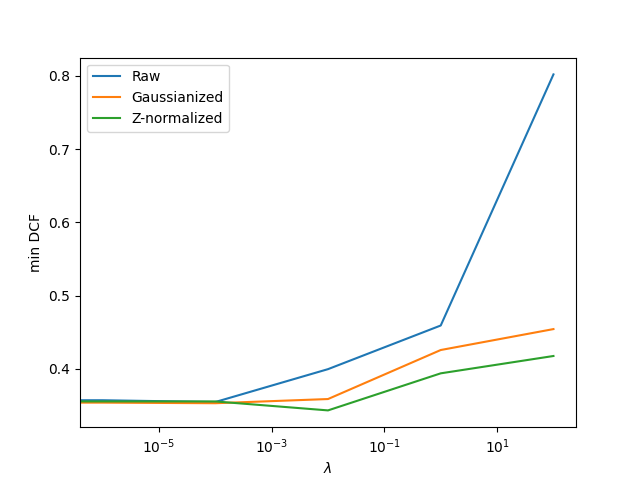
\includegraphics[width=.5\linewidth]{assets/logistic/lr_kfold_0.5.png}}
	\subfloat[linear, single split]{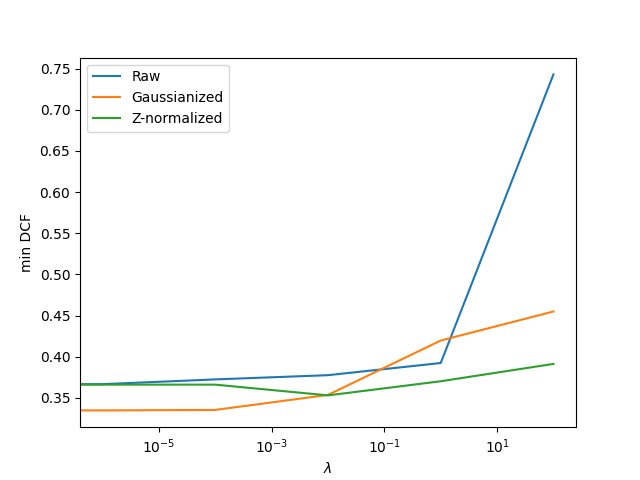
\includegraphics[width=.5\linewidth]{assets/logistic/lr_single_0.5.png}}\\
	\subfloat[quadratic, 5-fold]{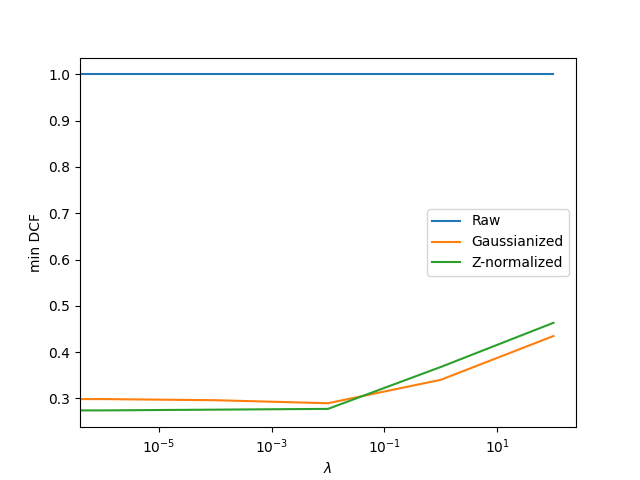
\includegraphics[width=.5\linewidth]{assets/logistic/qlr_kfold_0.5.png}}
	\subfloat[quadratic, single split]{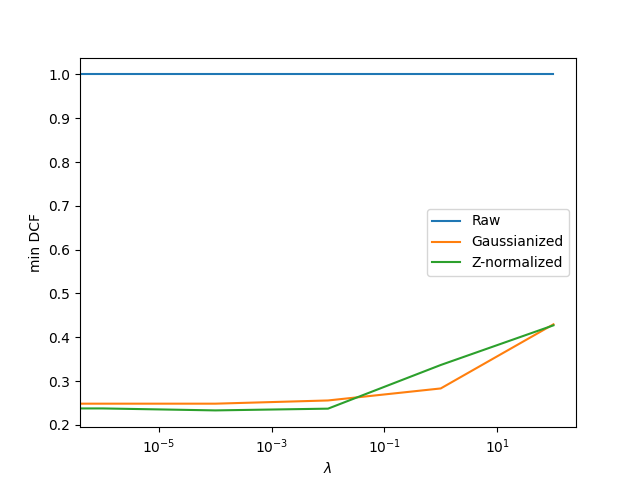
\includegraphics[width=.5\linewidth]{assets/logistic/qlr_single_0.5.png}}
	\caption{min DCF for Linear and Quadratic Logistic Regression over different values of $\lambda$}
	\label{fig:lr_plot}
\end{figure}

Differently from the previous case, Gaussianization doesn't prove this helpful, however standardizing data improved the performances. On the other hand, PCA does not bring any advantage, even if it doesn't prove detrimental.

Overall, among the different values of $\lambda$ and the two models in the 3 different scenario analysed, the quadratic logistic regression with $\lambda=0$ yields the best results. This is, to some extent, expected: quadratic models are characterized by a "curved" surface, which usually allow to better describe and learn the real distribution of the data, without overfitting.



%%%%%%%%%%%%%%%%%%%%%%%%%%%%%%%%%%%%%%%%%%%%     
%% Support Vector Classifier
%%%%%%%%%%%%%%%%%%%%%%%%%%%%%%%%%%%%%%%%%%%

\subsection{Support Vector Classifier}
In this section, we test the performances of 
different flavours of support vector classifiers. In particular, we are going to use a linear kernel, a quadratic polynomial kernel and a radial basis function (RBF) kernel.

\noindent
\begin{table}[H]
	\resizebox{.5\textwidth}{!}{
	\begin{tabular}{ p{5cm} P{1.9cm} P{1.4cm}  }
		\hline
		\hline
		& \makecell{\textbf{Single split} \\ $\tilde{\pi} = 0.5$} & \makecell{\textbf{5-fold} \\ $\tilde{\pi} = 0.5$} \\
		\hline
		\multicolumn{3}{c}{Raw features} \\
		\hline
		SVC($C=0.1$) & 0.816 & 0.760\\
		SVC($C=0.1, \pi^{emp}_T$) & 0.695 &  0.920\\
		\hline
		\multicolumn{3}{c}{Z-normalized features} \\
		\hline
		SVC($C=1$)   &\boxit{red}{1.3in} 0.334 & 0.341 \\
		SVC($C=0.1, \pi^{emp}_T$) & 0.338 & 0.348 \\
		\hline
		\multicolumn{3}{c}{Gaussianized features} \\
		\hline
		SVC($C=0.1$) & 0.339 & 0.350 \\
		SVC($C=0.1, \pi^{emp}_T$) & 0.352 & 0.360\\		
		\hline
	\end{tabular}
	}
	\caption{min DCF for Support Vector Classifier models, with and without feature balancing.}
	\label{tab:svc_res}
\end{table}

As done for the previous class of models, we will also take into account the possibility of rebalancing the classes introducing an empirical prior $\pi^{emp}_{T}$ over the training set, thus using two different values of $C$ for the bad and good quality wines
\begin{align*}
	C_T = C \cfrac{\pi_T}{\pi^{emp}_{T}} \ \ \ \ \ \
	C_F = C \cfrac{1 - \pi_T}{1 - \pi^{emp}_{T}} 
\end{align*}
We will first conduct our analysis emplying the linear SVC, even if we already discussed above that linear models don't perform that good for our classification task.
 
The best results obtained for the linear kernel are reported in Table \ref{tab:svc_res}, where we specified $\pi^{emp}_T$ where we balanced the features using the empirical prior. We observe that standardization improved greatly the results with respect to the raw case, where the classifier performs poorly both for the single split and the 5-fold approach. Conversely, Gaussianization and features balancing don't prove advantageous. A complete visualization is provided in Figure \ref{fig:svc_plot}.

A further analysis is, now, conducted using a polynomial kernel of grade 2 (quadratic) and a radial basis function (RBF) kernel. We tune again $C$ for both the cases and for the RBF kernel we perform a grid search involving $\gamma$ as well, to select the best hypermameters. Overall, we try the following values:
\begin{align*}
	C = \{10^{-1}, \ 1, \ 10\} \\
	\gamma = \{1/e, \ 1/e^2\} \\
	\pi_T = \{0.5, \ \pi^{emp}_T\}
\end{align*}
Place notice that $\pi_T$ is included above, even if it's not an hyperparameter, only to convey the idea that we're searching the best combination of parameters and, at the same time, assessing the benefits of rebalancing features, if any. A visualization of the grid is shown in Figure \ref{fig:kern_svc_plot}.

%% PLOTS here

\begin{figure}[H]
	%\centering
	\subfloat[balancing, 5-fold]{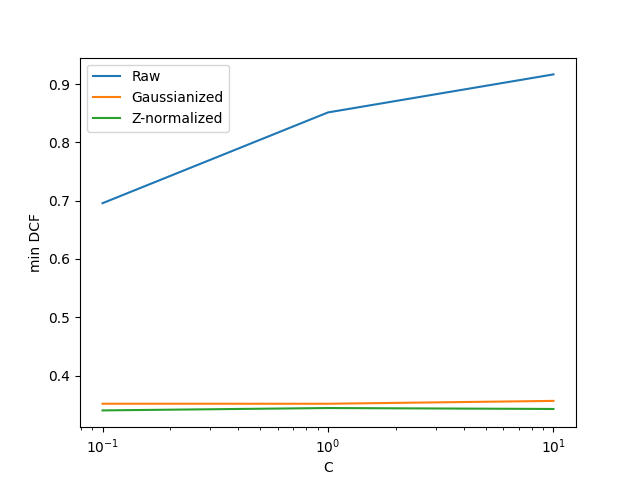
\includegraphics[width=.5\linewidth]{assets/svc_lin_kfold_bal.png}}
	\subfloat[no balancing, 5-fold]{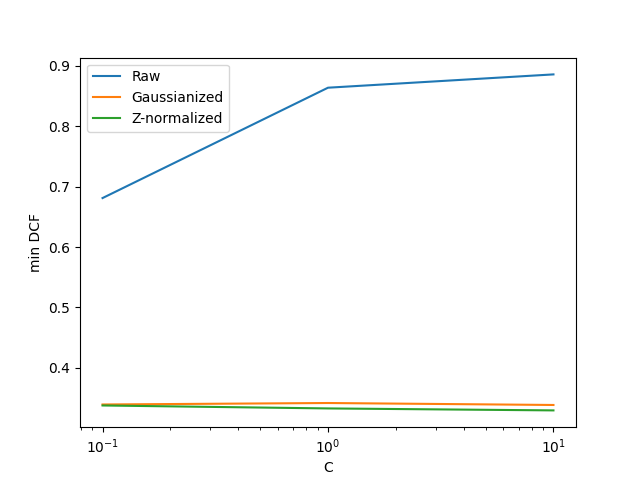
\includegraphics[width=.5\linewidth]{assets/svc_lin_kfold.png}}\\
	\subfloat[balancing, single split]{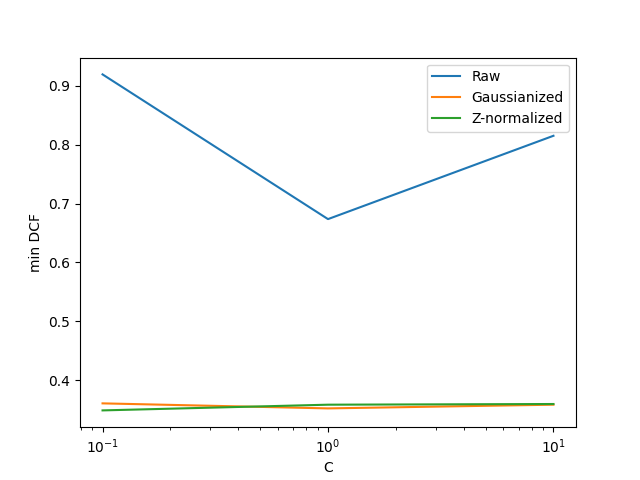
\includegraphics[width=.5\linewidth]{assets/svc_lin_single_bal.png}}
	\subfloat[no balancing, single split]{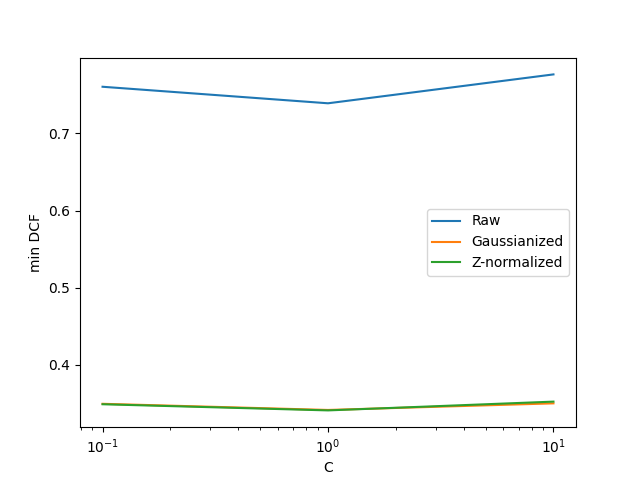
\includegraphics[width=.5\linewidth]{assets/svc_lin_single.png}}
	\caption{min DCF for Linear SVC with and without features balancing, over different values of $C$}
	\label{fig:svc_plot}
\end{figure}

We can notice that, for the RBF SVC, we obtain similar results regardless of features balancing. Therefore, balancing is not beneficial nor detrimental in our specific case. Table \ref{tab:best_svc_res} shows the results of the 2nd degree polynomial kernel and RBF kernel for the best choices of the hyperparameters, both with and without balancing.

\begin{figure}[H]
	%\centering
	\subfloat[quadratic SVC, 5-fold]{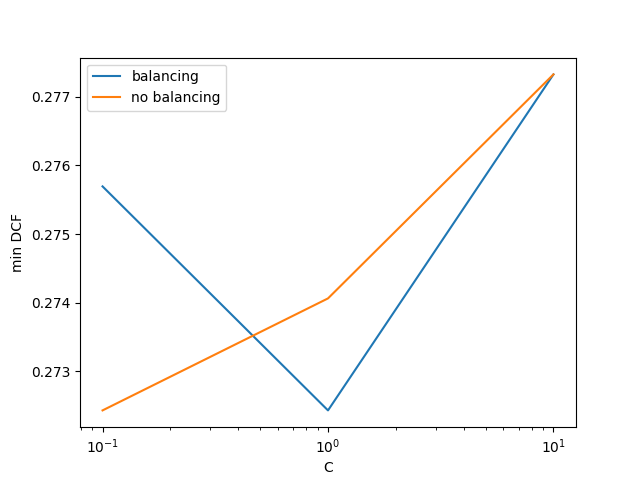
\includegraphics[width=.5\linewidth]{assets/quad_svc_kfold.png}}
	\subfloat[quadratic SVC, single split]{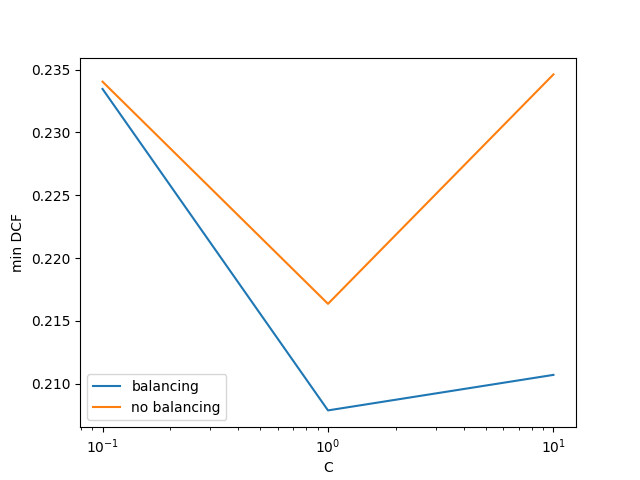
\includegraphics[width=.5\linewidth]{assets/quad_svc.png}}\\
	\subfloat[RBF SVC, 5-fold]{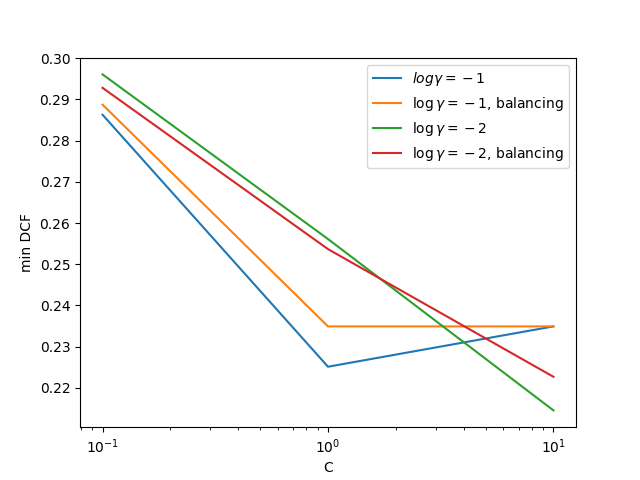
\includegraphics[width=.5\linewidth]{assets/svc_rbf_kfold.png}}
	\subfloat[RBF SVC, single split]{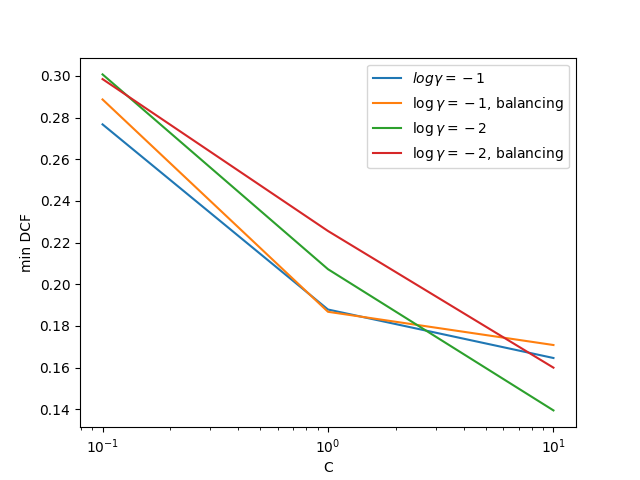
\includegraphics[width=.5\linewidth]{assets/svc_rbf_single.png}}
	\caption{min DCF for Quadratic and RBF SVC}
	\label{fig:kern_svc_plot}
\end{figure}



\noindent
\begin{table}[H]
	\resizebox{.5\textwidth}{!}{
	\begin{tabular}{ p{5.5cm} P{1.9cm} P{1.2cm}  }
		\hline
		\hline
		& \makecell{\textbf{Single split} \\ $\tilde{\pi} = 0.5$} & \makecell{\textbf{5-fold} \\ $\tilde{\pi} = 0.5$} \\
		\hline
		
		\multicolumn{3}{c}{Z-normalized features} \\
		\hline
		Poly-SVC($C=1$)  & 0.208 & 0.272 \\
		Poly-SVC($C=0.1, \pi^{emp}_T$) & 0.234 & 0.272 \\	
		RBF-SVC($C=10, log\gamma=-2$) & \boxit{red}{.35in}0.140 & \boxit{red}{.35in}0.215 \\
		RBF-SVC($C=10, log\gamma=-2, \pi^{emp}_T$) & 0.160 & 0.223 \\
		\hline
	\end{tabular}
	 }
	\caption{min DCF for Support Vector Classifier models, with and without feature balancing.}
	\label{tab:best_svc_res}
\end{table}

Overall, we can conclude that the RBF kernel yields the best results for the chosen metric. This model is, in addition, the most performing this far. 

%%%%%%%%%%%%%%%%%%%%%%%%%%%%%%%%%%%%%%%%%%%%
%% 		Gaussian Mixtures
%%%%%%%%%%%%%%%%%%%%%%%%%%%%%%%%%%%%%%%%%%%%
\subsection{Gaussian Mixture Models}
Eventually, Gaussian Mixtures are the last type of classifier employed for this task, for which we expect to yield generally better results than Gaussian models, as GMMs can approximate generic distributions.

We consider both full and diagonal covariance models, with and without covariance tying, where tying takes place at class level (i.e. different classes have different covariance matrices) for a total of 4 models. The best number of components is selected via cross-validation on gaussianized and standardized features. The results obtained for the described case are shown in Figure \ref{fig:gmm_plot}, where we preferred a line plot over a bar plot for a better visualization of the trend of the minimum DCF as the number of components increases.

\begin{figure}[H]
	%\centering
	\subfloat[Full GMM]{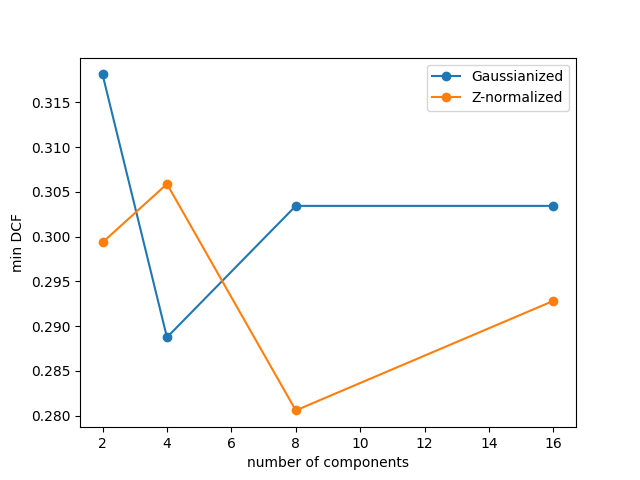
\includegraphics[width=.5\linewidth]{assets/gmm/gmm_full_0.5.png}}
	\subfloat[Diag GMM]{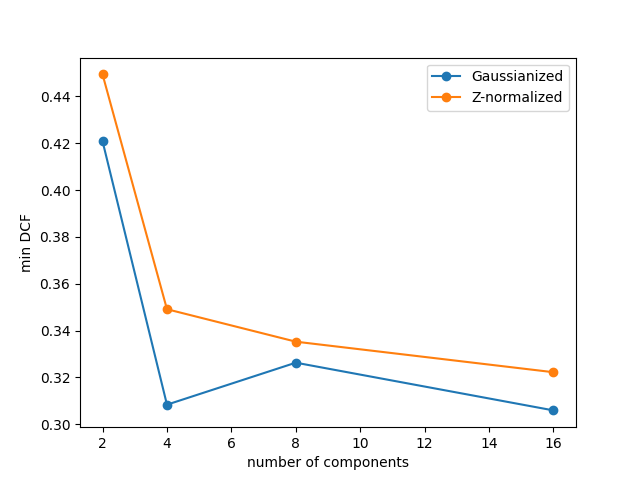
\includegraphics[width=.5\linewidth]{assets/gmm/gmm_diag_0.5.png}}\\
	\subfloat[Tied Full GMM]{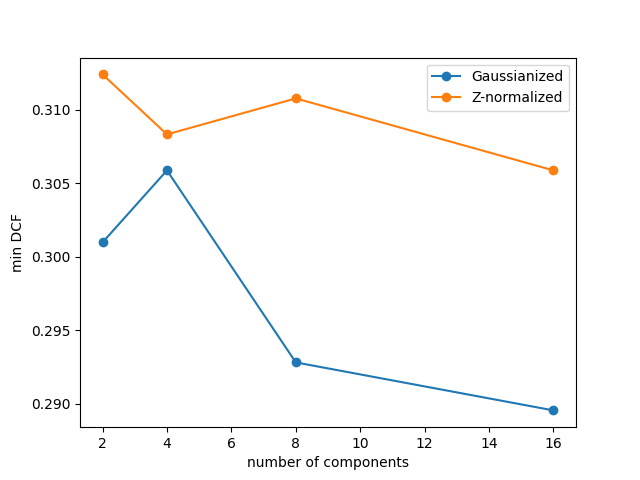
\includegraphics[width=.5\linewidth]{assets/gmm/gmm_full_tied_0.5.png}}
	\subfloat[Tied Diag GMM]{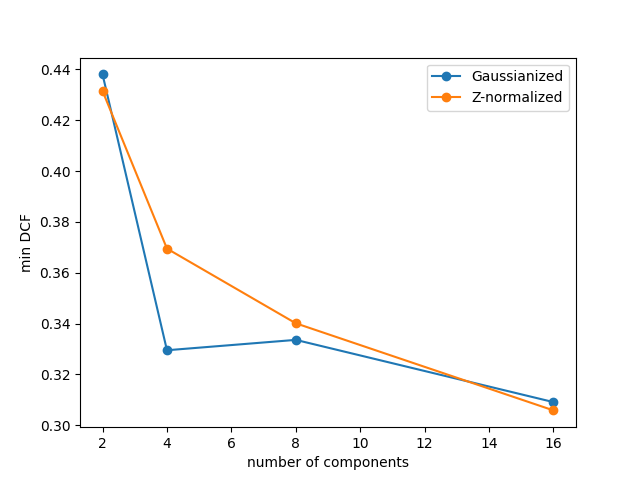
\includegraphics[width=.5\linewidth]{assets/gmm/gmm_diag_tied_0.5.png}}
	\caption{min DCF for different covariance types of Gaussian Mixtures Models}
	\label{fig:gmm_plot}
\end{figure}

\noindent
\begin{table}[H]
	\resizebox{.5\textwidth}{!}{
		\begin{tabular}{ p{5.4cm} P{1.2cm} P{1.2cm} P{1.2cm}}
			\hline
			\hline
			&  & \makecell{\textbf{5-fold}} 
			\\
			& $\tilde{\pi}=0.1$ & $\tilde{\pi}=0.5$ & $\tilde{\pi}=0.9$ \\
			\hline
			\multicolumn{2}{c}{Guassianized features} \\
			\hline
			Tied-GMM (4 components)       & 0.741                   & 0.306 & 0.754 \\
			GMM(8 components) 	          & 0.701 & 0.298 & 0.771 \\	
			Tied-Diag-GMM (16 components) & 0.714 					& 0.301 & 0.690 \\
			Diag-GMM (16 components)      & 0.694 					& 0.306 & \boxit{red}{.35in}0.634 \\
			\hline
			\multicolumn{2}{c}{Z-normalized features} \\
			\hline
			Tied-GMM (8 components)       & 0.769 					& 0.308                     & 0.842 \\
			GMM (8 components) 	          & \boxit{red}{.35in}0.689 & \boxit{red}{.35in}0.280   & 0.834 \\	
			Tied-Diag-GMM (16 components) & 0.752 					& 0.306 					& 0.793  \\
			Diag-GMM (16 components)      & 0.774 					& 0.322 					& 0.684\\
			\hline
		\end{tabular}
	}
	\caption{min DCF for Gaussian Mixture Models}
	\label{tab:gmm_res}
\end{table}

The above plot shows how for diagonal-covariance models (a, b) the min DCF decreases as the number of components increases, whereas it does not appear to be the case for full-covariance models. Table \ref{tab:gmm_res} reports the results for the selected models. We notice how the full-covariance GMM yields the minimum detection cost function when applied to Z-normalized features and, for the balanced prior application, provides valid results in order to conduct further analysis using this model. The overall scores of the 8-components full-cov GMM for the 3 applications are shown in Figure \ref{fig:gmm_pi} .



\begin{figure}[H]
	%\centering
	\subfloat[Gaussianized data]{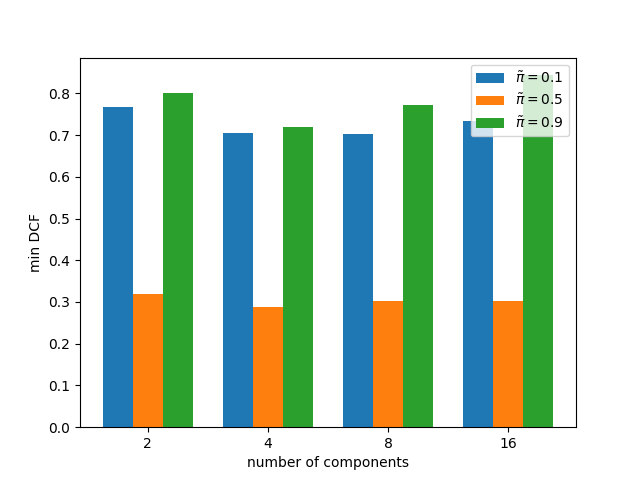
\includegraphics[width=.5\linewidth]{assets/gmm/gmm_gauss_pi.png}}
	\subfloat[Z-normalized data]{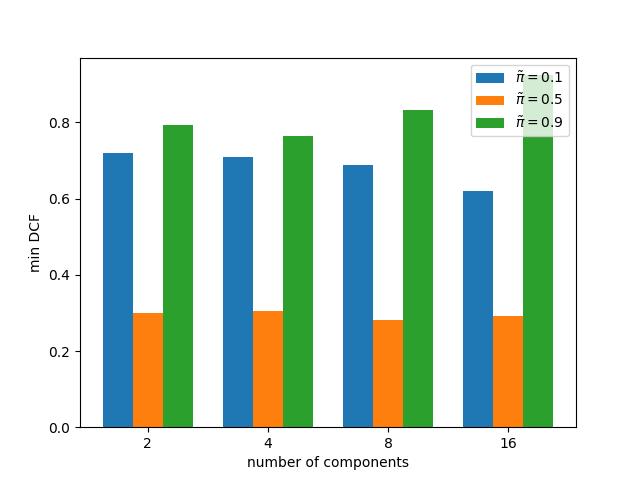
\includegraphics[width=.5\linewidth]{assets/gmm/gmm_std_pi.png}}
	\caption{min DCF for the full GMM over different priors and for different number of components}
	\label{fig:gmm_pi}
\end{figure}

\subsection{Model selection}
At the end of our preliminary analysis, we can conclude that the Support Vector Classifier with a radial basis function kernel having $log\gamma = -2$, applied to standardized features yields, globally, the best performances. 
Nevertheless, the Quadratic Logistic Regression and the Gaussian Mixture with 8 components - both applied to standardized features - performed well. We will mainly take these into account in the following analysis. 

To sum up, here are our best choices:
\begin{itemize}
	\item GMM(8 components)
	\item Quad-LR ($\lambda=0$)
	\item RBF SVC($log \gamma=-2$)
\end{itemize}
